\documentclass[letterpaper, reqno,11pt]{article}
\usepackage[margin=1.0in]{geometry}
\usepackage{color,latexsym,amsmath,amssymb,graphicx,float,listings,tikz}
\usepackage{hyperref}

\hypersetup{
colorlinks=true,
linkcolor=magenta,
filecolor=magenta,
urlcolor=cyan,
}

\lstset{
basicstyle=\ttfamily,
columns=fullflexible,
frame=single,
breaklines=true,
postbreak=\mbox{\textcolor{red}{$\hookrightarrow$}\space},
}

\graphicspath{ {images/} }

\begin{document}
\pagenumbering{arabic}
\title{PHYS 408 Homework 5}
\date{08/04/24}
\author{Xander Naumenko}
\maketitle

% {\medskip\noindent\bf Question 1a.} From equation 11.2-33 in Saleh \& Teich, we have
% \[
% \nu_{l,m,q} = q\nu_F+(l+m+1) \frac{\Delta\zeta}{\pi}\nu_F
% .\]
% Since the mirrors for the cavity weren't specified, I assume they're symmetric and so $\Delta\zeta=\zeta(z_0)-\zeta(-z_0)=\text{tan}^{-1}(1)-\text{tan}^{-1}(-1)=\frac{\pi}{2}$. Here $\nu_F=\frac{c}{2d}=\frac{3\cdot 10^{8}}{2\cdot 0.2}=750$GHz, and the frequency band for $\lambda=500\pm 0.1$nm is $\nu=600.12$ to 599.88THz. Applying these bounds, we have
% \[
% 599.88\leq 0.75\left(q+\frac{1}{2}\left( l+m+1 \right) \right)\leq 600.12
% .\]
% \[
% \implies 799.84\leq q+\frac{1}{2}\left( l+m+1 \right) \leq 800.16\implies q+\frac{1}{2}(l+m+1)=800
% .\]
% Now this is just a combinatorics problem. For a fixed value of $q$, There are $2(800-q)$ ways for $\frac{1}{2}(l+m+1)=800-q$, so we have
% \[
% \#\text{ Modes}=\sum_{q=0}^{800}2(800-q)=640800
% .\]

{\medskip\noindent\bf Question 1a.} From in class, we have that the density of cavity modes is $\frac{8\pi}{\lambda^3\nu}$. For a spectral range of 0.1nm, we that the number of cavity modes is approximately
\[
\#\text{ Modes}=\frac{8\pi}{\lambda^3\nu}\cdot 120\cdot 10^{9}\cdot 0.2\cdot 0.1=8.04\cdot 10^{14}
.\]

{\medskip\noindent\bf Question 1b.} The spectral width range goes from $499.95$ to $500.05$nm, so it is of width $\Delta\nu=c \left( \frac{1}{499.95\cdot 10^{-9}}-\frac{1}{500.05\cdot 10^{-9}} \right)=120$GHz. The number of TEM$_{q,0,0}$ modes will be approximately the spectral width divided by the FSR, where $\nu_F=\frac{c}{2d}=750$MHz, so $2\frac{\Delta\nu}{\nu}=320$.

{\medskip\noindent\bf Question 1c.} Assuming each mode is equally likely, we get that the probability is $\frac{320}{8.04\cdot 10^{14}}=3.98\cdot 10^{-13}$.

{\medskip\noindent\bf Question 1d.} Using the cross section formula:
\[
\sigma= \frac{\gamma_{sp}\lambda^2}{4\Delta\omega}=5.2\cdot 10^{-18}\text{m}
.\]

% {\medskip\noindent\bf Question 2a.} Using the relations derived in class we can solve for $I_{sat}$:
% \[
% I^{(out)}=I^{(in)}e^{g_0L}\implies g_0=\frac{1}{L}\log \frac{I^{(out)}}{I^{(in)}}
% .\]

{\medskip\noindent\bf Question 2a.} From in class, we have the following relation:
\[
\log \frac{I_2}{I_1}+\frac{I_2-I_1}{I_{sat}}=g_0l_g
.\]
Since $g_0l_g$ are the same in both cases, we can solve for $I_{sat}$:
\[
\log 10+ \frac{9}{I_{sat}}=\log 7.5+\frac{13}{I_{sat}}\implies I_{sat}=13.9\text{W/cm}^2
.\]
{\medskip\noindent\bf Question 2b.} Using this same equation to solve for $g_0$:
\[
g_0= \frac{1}{l_g}\left( \log \frac{I_2}{I_1}+\frac{I_2-I_1}{I_{sat}} \right)=2.95\text{cm}^{-1}
.\]

{\medskip\noindent\bf Question 2c.} Again using the formula derived in class:
\[
I_{ss}=I_{sat} \frac{g_0}{a}=3.01 \frac{5.29}{0.01 /1}=4100.5\text{W/cm}^2
.\]

{\medskip\noindent\bf Question 2d.} Using $I_{2}=I_{ss}/2$ and solving for $I_1$, we can solve the following equation numerically:
\[
\log \frac{I_{ss}}{2I_1}+ \frac{I_{ss}-2I_1}{2I_{sat}}=g_0l_g\implies I_1=2009.5\text{W/m}^2
.\]

{\medskip\noindent\bf Question 2e.} Again, we derived expressions for both of these values in class:
\[
T^{(opt)}_{oc}=\sqrt{g_0l_ga}-a=0.162
.\]
\[
I^{(opt)}_{out}=I_{sat}\left( \sqrt{g_0l_g}-\sqrt{a} \right) ^2=36.4
.\]

{\medskip\noindent\bf Question 3a.} For question 3, as question suggests we use the weak pump approximation. This means that $R_{p}\tau\ll 1$, and so $g(I)= \frac{g_{0,weak}}{1+I/I_{sat}}$. Note that $g\propto N_2$ and $P\propto N_2$, so $\frac{g(I)}{g_{0,weak}}=\frac{P_l}{P_0}$ (since $g_{0,weak}$ and $P_0$ are when no lasing occurs, while $g(I)$ and $P_0$ are for when it does). Plugging this into the original equation:
\[
P_l=\frac{P_0}{1+I /I_{sat}}
.\]

{\medskip\noindent\bf Question 3b.} We can relate $I_{out}$ with $I_{2}$ with $I_2=\frac{I_{out}}{T_{oc}}=100$W/cm$^{2}$. Plugging into part a:
\[
1=\frac{2}{1+100 /I_{sat}}\implies I_{sat}=I_{sat}=100\text{W/cm}^2
.\]

{\medskip\noindent\bf Question 4a.} Rate equations:
\[
\dot N_1=A_{21}N_2+R_{13}\left( N_3-N_1 \right) 
\]
\[
\dot N_2=A_{32}N_3-A_{21}N_2 
\]
\[
\dot N_3=-A_{32}N_3-R_{13}\left( N_3-N_1 \right) 
.\]
Using $N=N_3+N_2+N_1$:
\[
\dot N_1=A_{21}N_2+R_{13}\left( N-2N_1-N_2 \right) 
\]
\[
\dot N_2=A_{32}(N-N_1-N_2)-A_{21}N_2 
.\]
Substituting given constants:
\[
\dot n_1=n_2+R\left( 1-2n_1-n_2 \right) 
\]
\[
\dot n_2=aR\left( 1-n_1-n_2 \right) -n_2
.\]

{\medskip\noindent\bf Question b.} Setting $\dot n_{1,2}=0$ and solving is a system of two linear equations with two unknowns, which gives:
\[
    n_1= \frac{a+1}{aR+a+2}, n_2= \frac{aR}{aR+a+2}\implies \Delta n=\frac{a(R-1)-1}{a(R+1)+2}
.\]

{\medskip\noindent\bf Question c.} It is a similar form as $\frac{R-1}{R+1}$, although with extra terms of $-1$ and $+2$. When $a$ is large it reduces to the form we saw in class though. To calculate $a_{10\%}$, we can solve directly (because the new form makes the numerator smaller and the denominator bigger we know that the real value will be lower than the in class estimate):
\[
\frac{a(R-1)-1}{a(R+1)+2}=0.9 \frac{R-1}{R+1}\implies \frac{a-1}{3a+2}=0.3\implies a_{10\%}=16
.\]

{\medskip\noindent\bf Question d.} See figure \ref{fig:q4d}, the parameters used were $R=2$ and $a=16$ as calculated. As expected, the equilibrium settles to within $10\%$ of the theoretical value. The code used for it was:
\begin{lstlisting}
import numpy as np
from scipy.integrate import solve_ivp
import matplotlib.pyplot as plt

R = 2
a = 16

F = lambda t,n: np.array([n[1]+R*(1-2*n[0]-n[1]), a*R*(1-n[0]-n[1])-n[1]])
t_eval = np.arange(0, 4.01, 0.01)

sol = solve_ivp(F, [0,4], [1, 1], t_eval=t_eval)

plt.plot(t_eval, sol.y.T[:,0], label='$n_1$')
plt.plot(t_eval, sol.y.T[:,1], label='$n_2$')
plt.axhline(y=(R-1)/(R+1)+sol.y.T[:,0][-1], color='g', linestyle='-', label='$\\frac{R-1}{R+1}$')
plt.axhline(y=(R-1)/(R+1)*0.9+sol.y.T[:,0][-1], color='y', linestyle='-', label='$\\pm 10\%$')
plt.legend()
plt.title('Numerical Solution to Three Level Lasing System')
plt.xlabel('Time (s)')
plt.ylabel('Scaled number in level')
plt.show()

\end{lstlisting}

\begin{figure}[htpb]
    \centering
    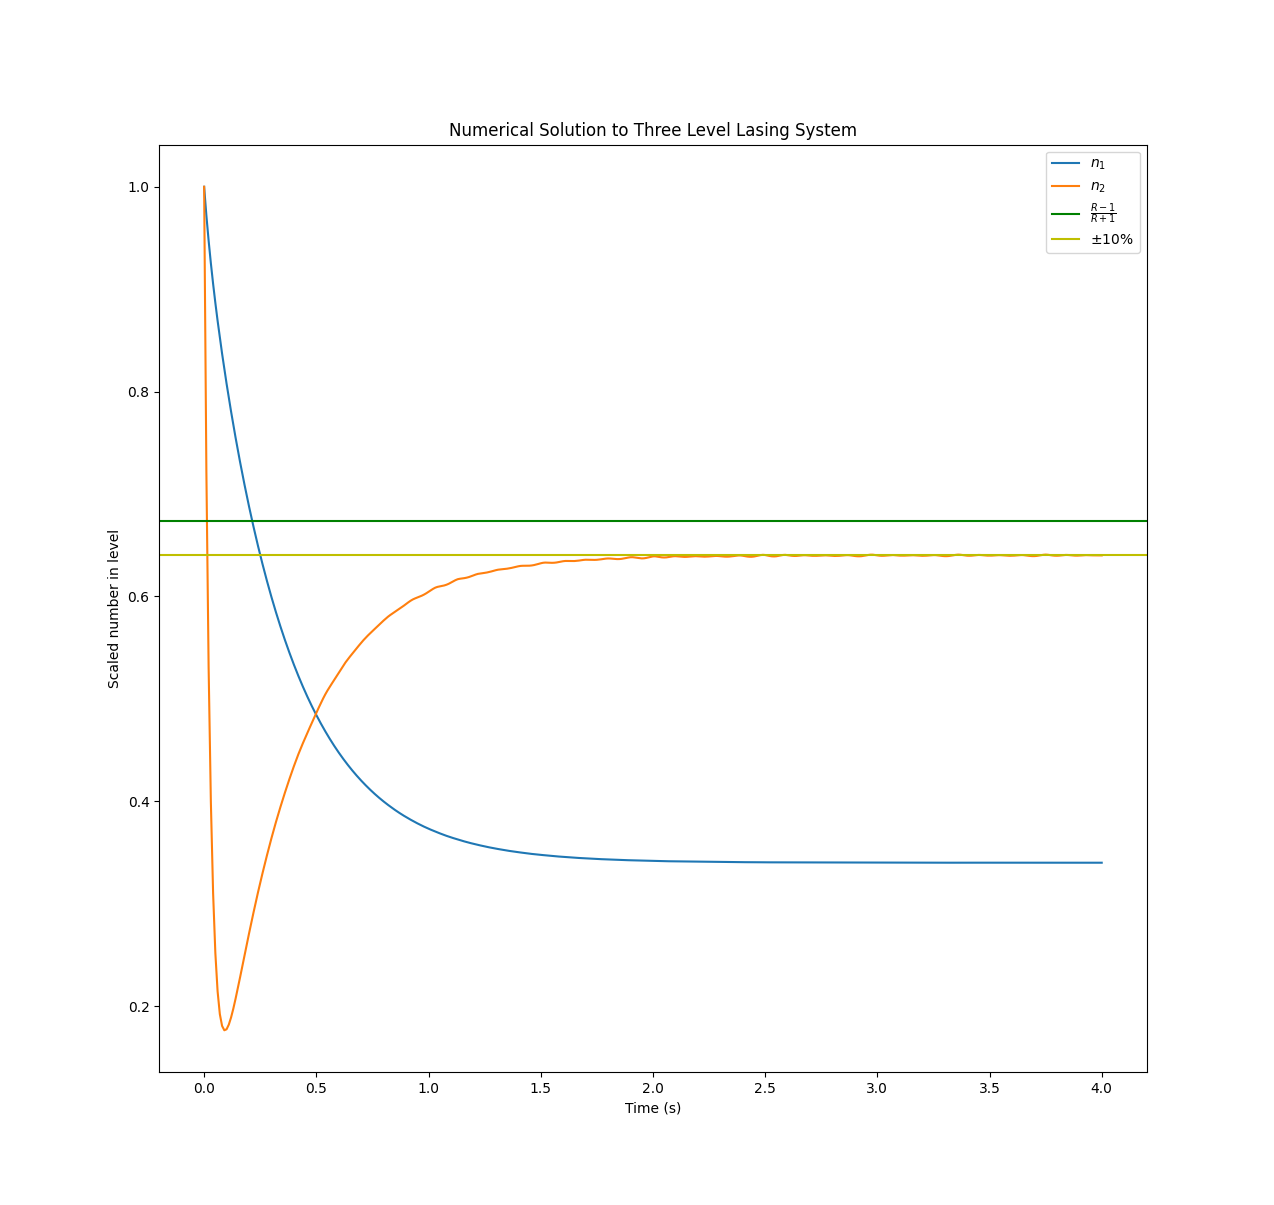
\includegraphics[width=0.8\textwidth]{q4}
    \caption{Numerical solution for question 4d. Arbitrary scaling for time and number, parameters used were $R=2$ and $a=16$.}
    \label{fig:q4d}
\end{figure}

\end{document}
